\section{Evaluation}\label{sec:eval}
We separate zero-LLM-call deterministic audits from bounded stochastic proposer pilots; cohorts and denominators are never pooled across lanes.

\subsection{E1 Offline Conformance and Deterministic Boundary Audit}
In \textbf{E1} (13 gate fixtures and 12 repair cases per arm), all four arms satisfy construction invariants (13/13 gate agreement, 10/10 integrity fault detections). On invalid repair fixtures, \texttt{rejection\_only} and \texttt{unchanged\_retry} recover 0/12, guided repair $\rho$ recovers 5/12 without reading \texttt{WorldState}, and the nondeployable state-reading oracle recovers 6/12.

To test authorization beyond single-world fixtures, our deterministic boundary audit crosses two room counts (4, 8), two topologies (locked chain, unlocked bypass branch), four start/goal placements of two reusable keys, and two quest stages ($2{\times}2{\times}4{\times}2=32$ configurations) with 13 candidate variants each (416 assignments/arm; 1,664 total) plus 48 surface-sentinel assignments (12/arm). An implementation-separated reference evaluates initial and repaired candidates against the immutable pre-action state using standard-library BFS reachability.

\begin{table}[!tbp]
\caption{Deterministic Authorization-Boundary Audit (416 Cases/Arm + 48 Surface Sentinels; 0 LLM Calls)}
\label{tab:boundary-full}
\centering
\footnotesize
\begin{tabularx}{\columnwidth}{@{}>{\raggedright\arraybackslash}X*{4}{>{\centering\arraybackslash}p{0.125\columnwidth}}@{}}
\toprule
\textbf{Outcome (416/arm)} & \textbf{Schema only} & \textbf{Sem.\ reject} & \textbf{Unch.\ retry} & \textbf{Guided $\rho$} \\
\midrule
Invalid initial proposals & 260 & 260 & 260 & 260 \\
Unsafe final commits & 260 & \textbf{0} & \textbf{0} & \textbf{0} \\
Repaired invalid $\rightarrow$ valid & 0 & 0 & 0 & \textbf{128} \\
Held (unchanged fallback) & 0 & 260 & 260 & 132 \\
Goal reached & 124 & 124 & 124 & \textbf{252} \\
Valid preserved (156 valid) & 156 & 156 & 156 & 156 \\
Signature retention (11 sigs) & 11/11 & 11/11 & 11/11 & 11/11 \\
\bottomrule
\end{tabularx}
\end{table}

Table~\ref{tab:boundary-full} shows that \texttt{schema\_only} committed all 260/416 reference-invalid proposals, whereas every semantic-gate arm recorded 0/416 unsafe commits, 0/156 false rejections, and 32/32 closure--BFS agreement. Guided repair $\rho$ recovered 128/260 invalid proposals, raising goal attainment from 124/416 to 252/416. On the 12/arm surface sentinels, all semantic gates blocked 6/6 explicit forbidden-fact declarations but admitted 6/6 undeclared paraphrases, quantifying the declared-field boundary.

\subsection{Disclosure Parity, NPC Screening, and KG Simulation}
On 60 authored \texttt{reveal\_hint} cases (48 normal, 4 boundary, 8 malformed; Fig.~\ref{fig:disclosure-signals}), an unchecked baseline produced 51 unique unsafe disclosures (60/60 allow), whereas \texttt{general\_rule} and \texttt{ontology\_gate} agreed on 60/60 outcomes (16 allow, 44 deny, 0 unsafe, 0 replay mismatches), establishing zero-regression audit binding rather than ontology superiority. Separately, deterministic \texttt{NPC-ENG1} (16 cases) and historical \texttt{NPC-SCR1} (72 rows; 24/arm, 20/24 complete, 4/24 goal, 12 stale-control ACK rejections) verify protocol state transitions and replay. In the closed-world KG link-proposal simulation (43 OKF nodes, 106 reference edges, 24 curated typed edges, 6 withheld-edge queries), typed-lexical retrieval (\texttt{S2}) achieved $P{=}R{=}1.000$, $\mathrm{MRR}{=}0.944$, and $\mathrm{Sem@3}{=}1.000$ versus degree baseline $P{=}R{=}0.000$ and $\mathrm{MRR}{=}0.282$.

\begin{figure}[!tbp]
\centering
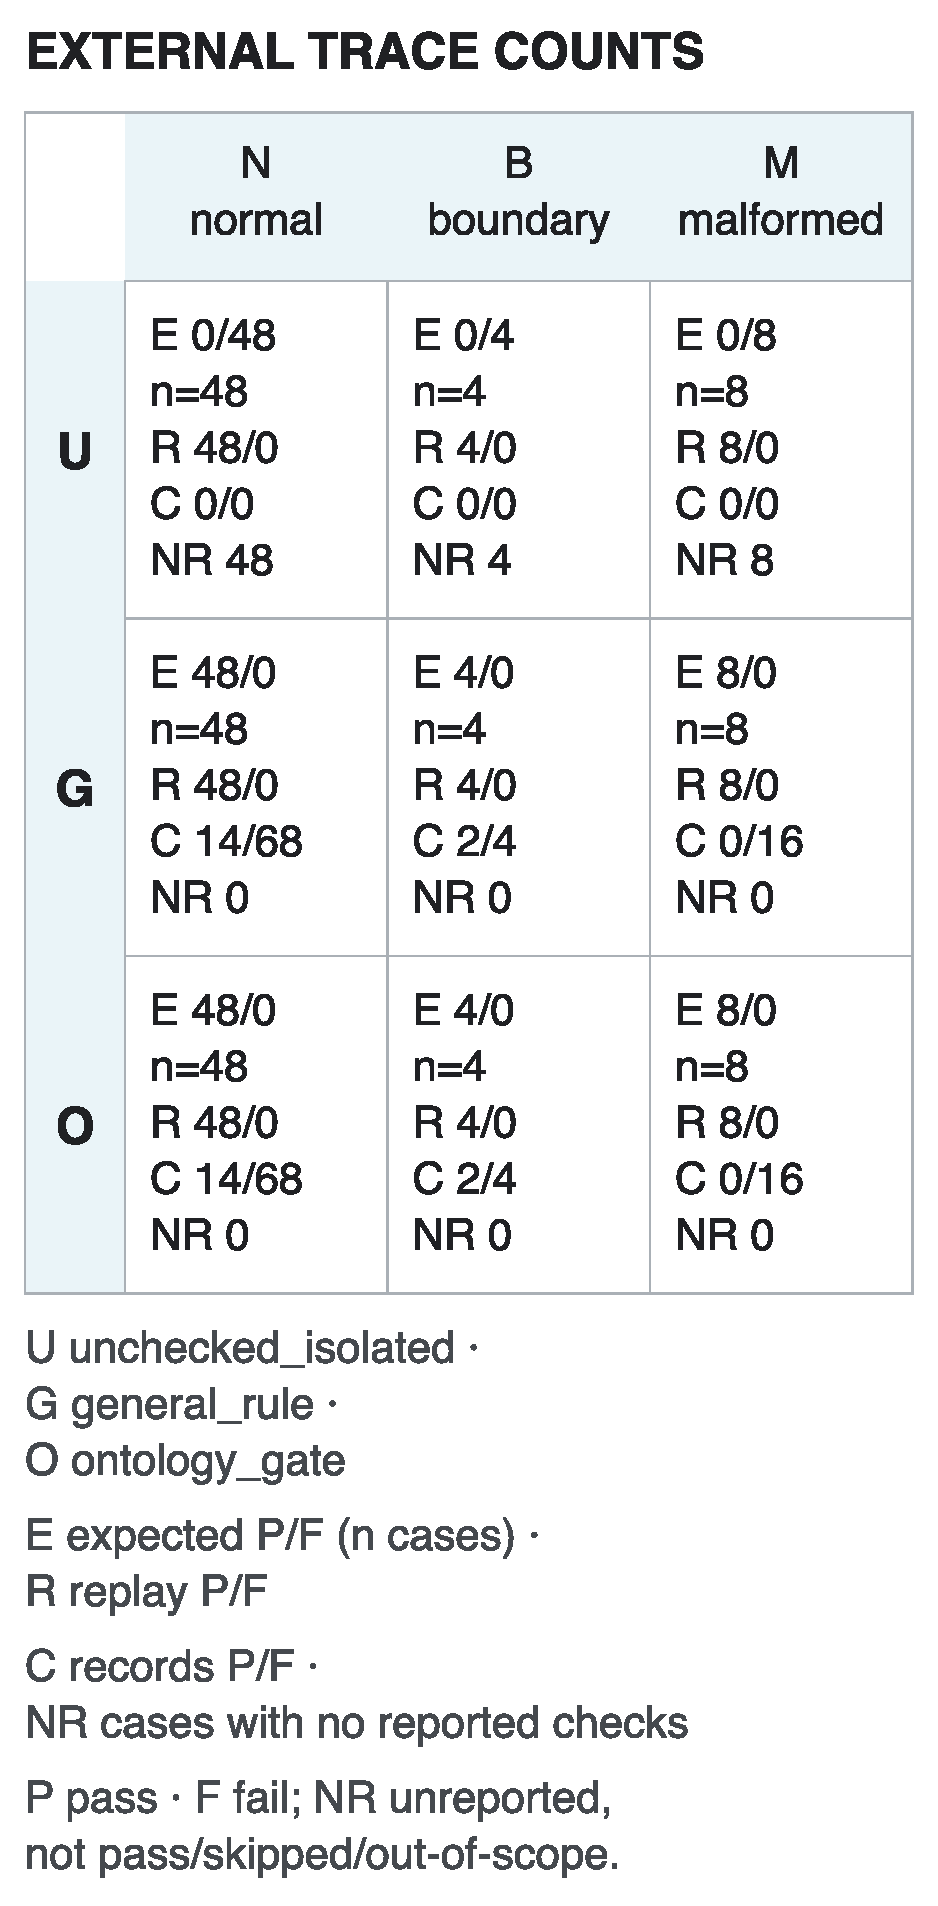
\includegraphics[width=\columnwidth]{../../figures/fig_disclosure_signals.pdf}
\caption{NPC-DISC-1 counts by arm and stratum (E/R: expectation match and replay; C: policy check PASS/FAIL; NR: no reported check).}
\Description{Bar matrix of NPC-DISC-1 counts by experimental arm and stratum comparing expectation match, replay, policy PASS/FAIL, and unreported checks.}
\label{fig:disclosure-signals}
\end{figure}

\subsection{Extended Zero-LLM Engineering Audits (A1--A4, B)}
Table~\ref{tab:extended-full} summarizes five independent-denominator deterministic audits covering multi-error repair convergence, latency scaling, seeded traceability sensitivity, Godot~4.7.1 soak stability (Fig.~\ref{fig:engine-cutscenes}), and secondary escape filtering.

\begin{table*}[!tbp]
\caption{Independent-Denominator Zero-LLM Engineering Audits (A1--A4, B)}
\label{tab:extended-full}
\centering
\footnotesize
\begin{tabularx}{\textwidth}{@{}>{\raggedright\arraybackslash}p{0.20\textwidth}>{\raggedright\arraybackslash}p{0.21\textwidth}>{\raggedright\arraybackslash}X@{}}
\toprule
\textbf{Audit} & \textbf{Denominator / Scope} & \textbf{Verified Deterministic Results (0 LLM Calls)} \\
\midrule
\textbf{A1} Multi-Error Convergence & 352 cases/budget ($K{\in}\{0..3\}$, 1,408 runs) + 128 guards & Safe commits: $K{=}0$ 0/352, $K{\ge}1$ 124/352 (35.23\%, unsafe 0/1,408); \texttt{repairable\_multi} 96/96 at $K{=}1$; \texttt{mixed\_partial\_clear} 28/160 at $K{=}1$, 132/160 held; \texttt{conflict\_pair} 0/96 cross-attempt commits (96/96 period-2 oscillation at $K{=}3$) vs.\ 128/128 same-pass conflict-guard freeze. \\
\textbf{A2} Scaling Benchmark & $N{\in}[10,2000]$ facts ($\text{arity}{\le}100$ above 500), $R{\in}[4,256]$ rooms & At $N{=}2000$: validator p95 0.0042\,ms (valid) / 0.0751\,ms (multi-error); $\rho$ p95 0.0317--0.0389\,ms; $R{=}256$ closure/BFS p95 0.312--0.478\,ms; SHA-256 verify 7.01\,ms; JSONL replay ($N{=}100,L{=}100$) 881.0\,ms. \\
\textbf{A3} Traceability Faults & 4,656 seeded faults (+1,584 N/A), 3,744 invariance, \texttt{TR05} map & Seeded sensitivity 4,656/4,656 (100.00\%); invariance false alarms 0/3,744 (0.00\%); \texttt{TR05} forward 12/12, reverse 10/10 direct files; human Krippendorff $\alpha$ unmeasured (0 human raters). \\
\textbf{A4} Godot~4.7.1 Soak & 11 refusals + 1,600 ticks (200 episodes) & Refusal codes 9/9 (100\%) exercised; state isolation 11/11; trace consistency 1,600/1,600; \texttt{step\_commit} p95 0.708\,ms; static memory delta $-268$\,B; 0 leaks. \\
\textbf{B} Escape Filter (EN/KO) & 88 cases (44 EN, 44 KO; \texttt{keeper\_secret}) & Recall / benign FRR / warm p95: ID-only 0.0\% / 0.0\% / 0.032\,ms; Alias 61.1\% (22/36) / 11.1\% (4/36) / 0.041\,ms; LOO TF-IDF 97.2\% (35/36) / \textbf{58.3\% (21/36)} / 0.705\,ms. \\
\bottomrule
\end{tabularx}
\end{table*}

\begin{figure*}[!tbp]
\centering
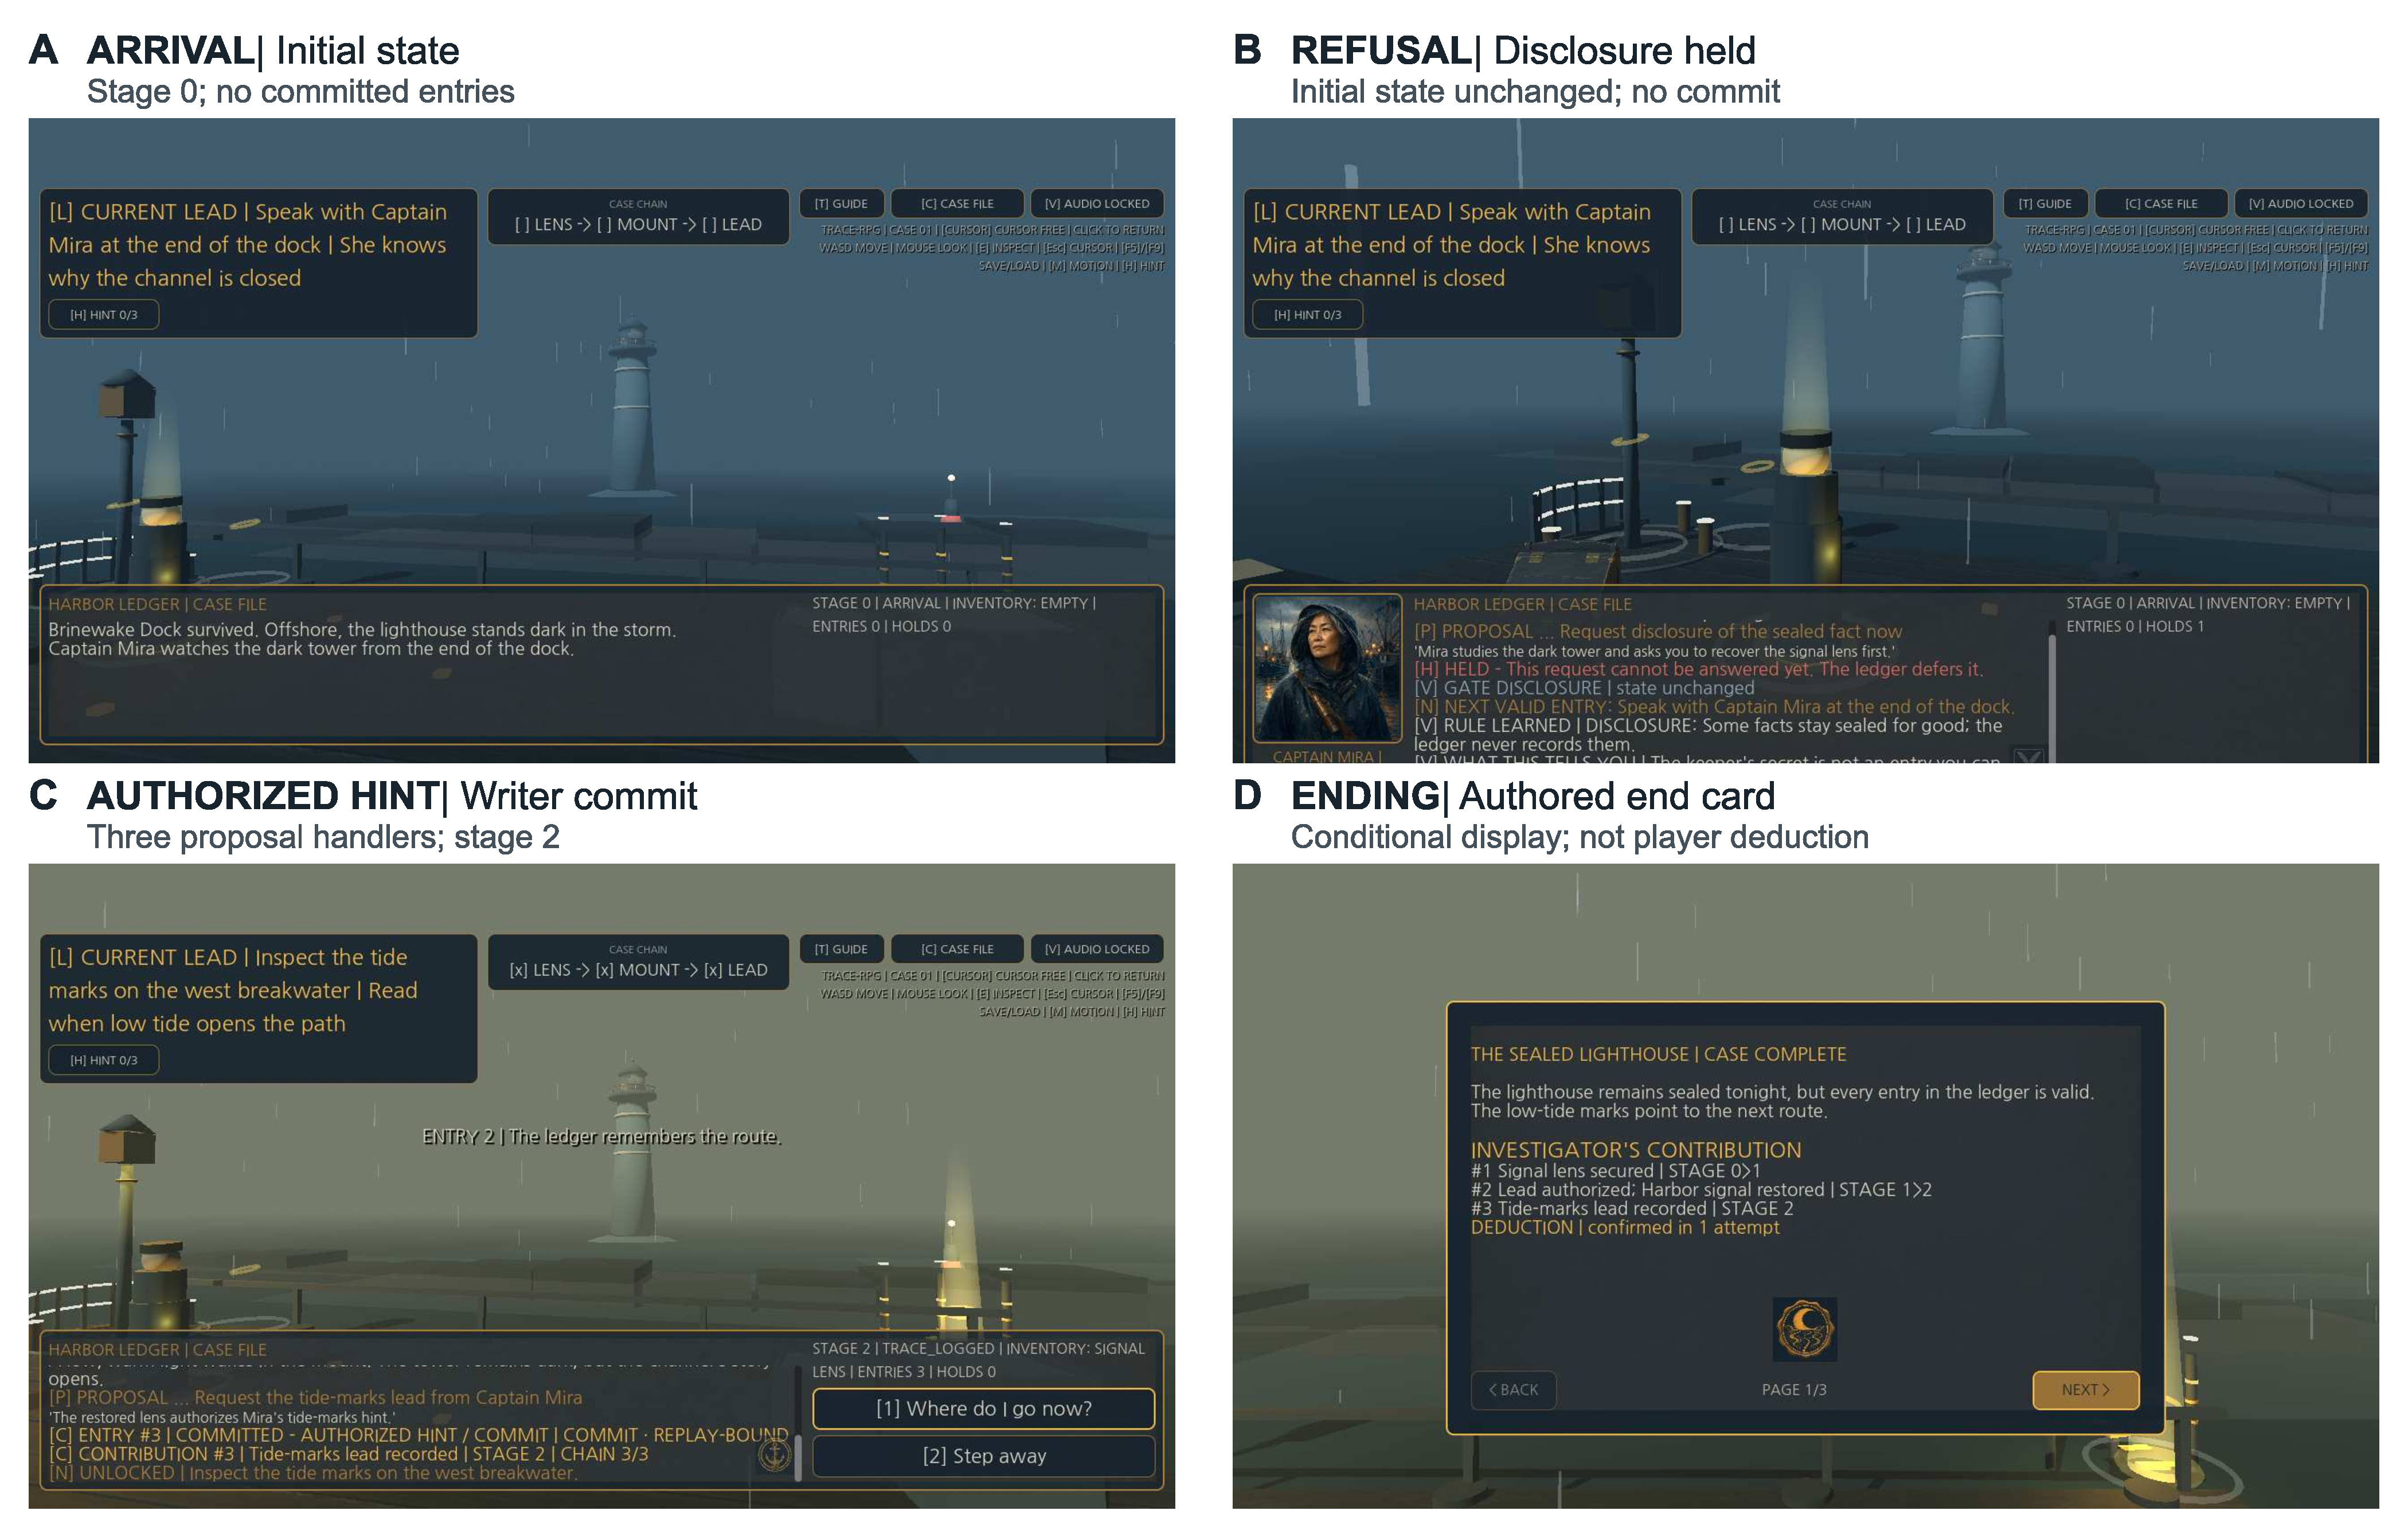
\includegraphics[width=0.92\textwidth]{../../figures/fig_engine_cutscenes.pdf}
\caption{Native Godot~4.7.1 engineering captures: (A) initial arrival; (B) denied secret disclosure leaving state unchanged; (C) authorized hint at stage 2; (D) conditional closing card. These captures verify rendered state correspondence rather than user efficacy.}
\Description{Four-panel Godot 4.7.1 screenshot sequence showing initial arrival, denied secret disclosure with unchanged state, stage-2 authorized hint, and closing card.}
\label{fig:engine-cutscenes}
\end{figure*}

\subsection{Bounded Stochastic Proposer Pilots}
In the \textbf{v5 two-stage collection} (20 assignments: 5 synthetic fixtures $\times$ 2 selectors $\times$ Detailed/Generic, $K{=}0$), 20/20 responses arrived, 10/20 passed strict parsing (Luna 9/10; Terra 1/10), 8/20 passed the semantic gate (Table~\ref{tab:v5-summary}, Fig.~\ref{fig:paired-feedback-flow}), and 7/20 reached \texttt{signal\_restored}; all 2 rejected parsed candidates fell back with zero state mutation. In the \textbf{native fixed-quest pilot} (8 assignments on \texttt{sealed-\allowbreak lighthouse-\allowbreak v1}), 5/8 reached the goal with 0/16 unsafe commits, 7/7 semantic replays valid, and 6/6 committed fresh Godot re-executions valid (1 pre-response controller-v3 serialization fault fixed to v4 in rows 2--8; 2 ontology rows timed out at 60\,s).

\begin{table}[!tbp]
\caption{v5 Synthetic Collection (5 Assigned Cases/Cell; Failures Retained)}
\label{tab:v5-summary}
\centering
\footnotesize
\begin{tabularx}{\columnwidth}{@{}ll*{4}{>{\centering\arraybackslash}X}@{}}
\toprule
\textbf{Selector} & \textbf{Signal} & \textbf{Recv} & \textbf{Gate} & \textbf{Goal} & \textbf{Parse Fail} \\
\midrule
\texttt{gpt-5.6-luna} & Detailed & 5/5 & 4/5 & 3/5 & 1/5 \\
\texttt{gpt-5.6-luna} & Generic  & 5/5 & 3/5 & 3/5 & 0/5 \\
\texttt{gpt-5.6-terra} & Detailed & 5/5 & 0/5 & 0/5 & 5/5 \\
\texttt{gpt-5.6-terra} & Generic  & 5/5 & 1/5 & 1/5 & 4/5 \\
\bottomrule
\end{tabularx}
\end{table}

\begin{figure}[!tbp]
\centering
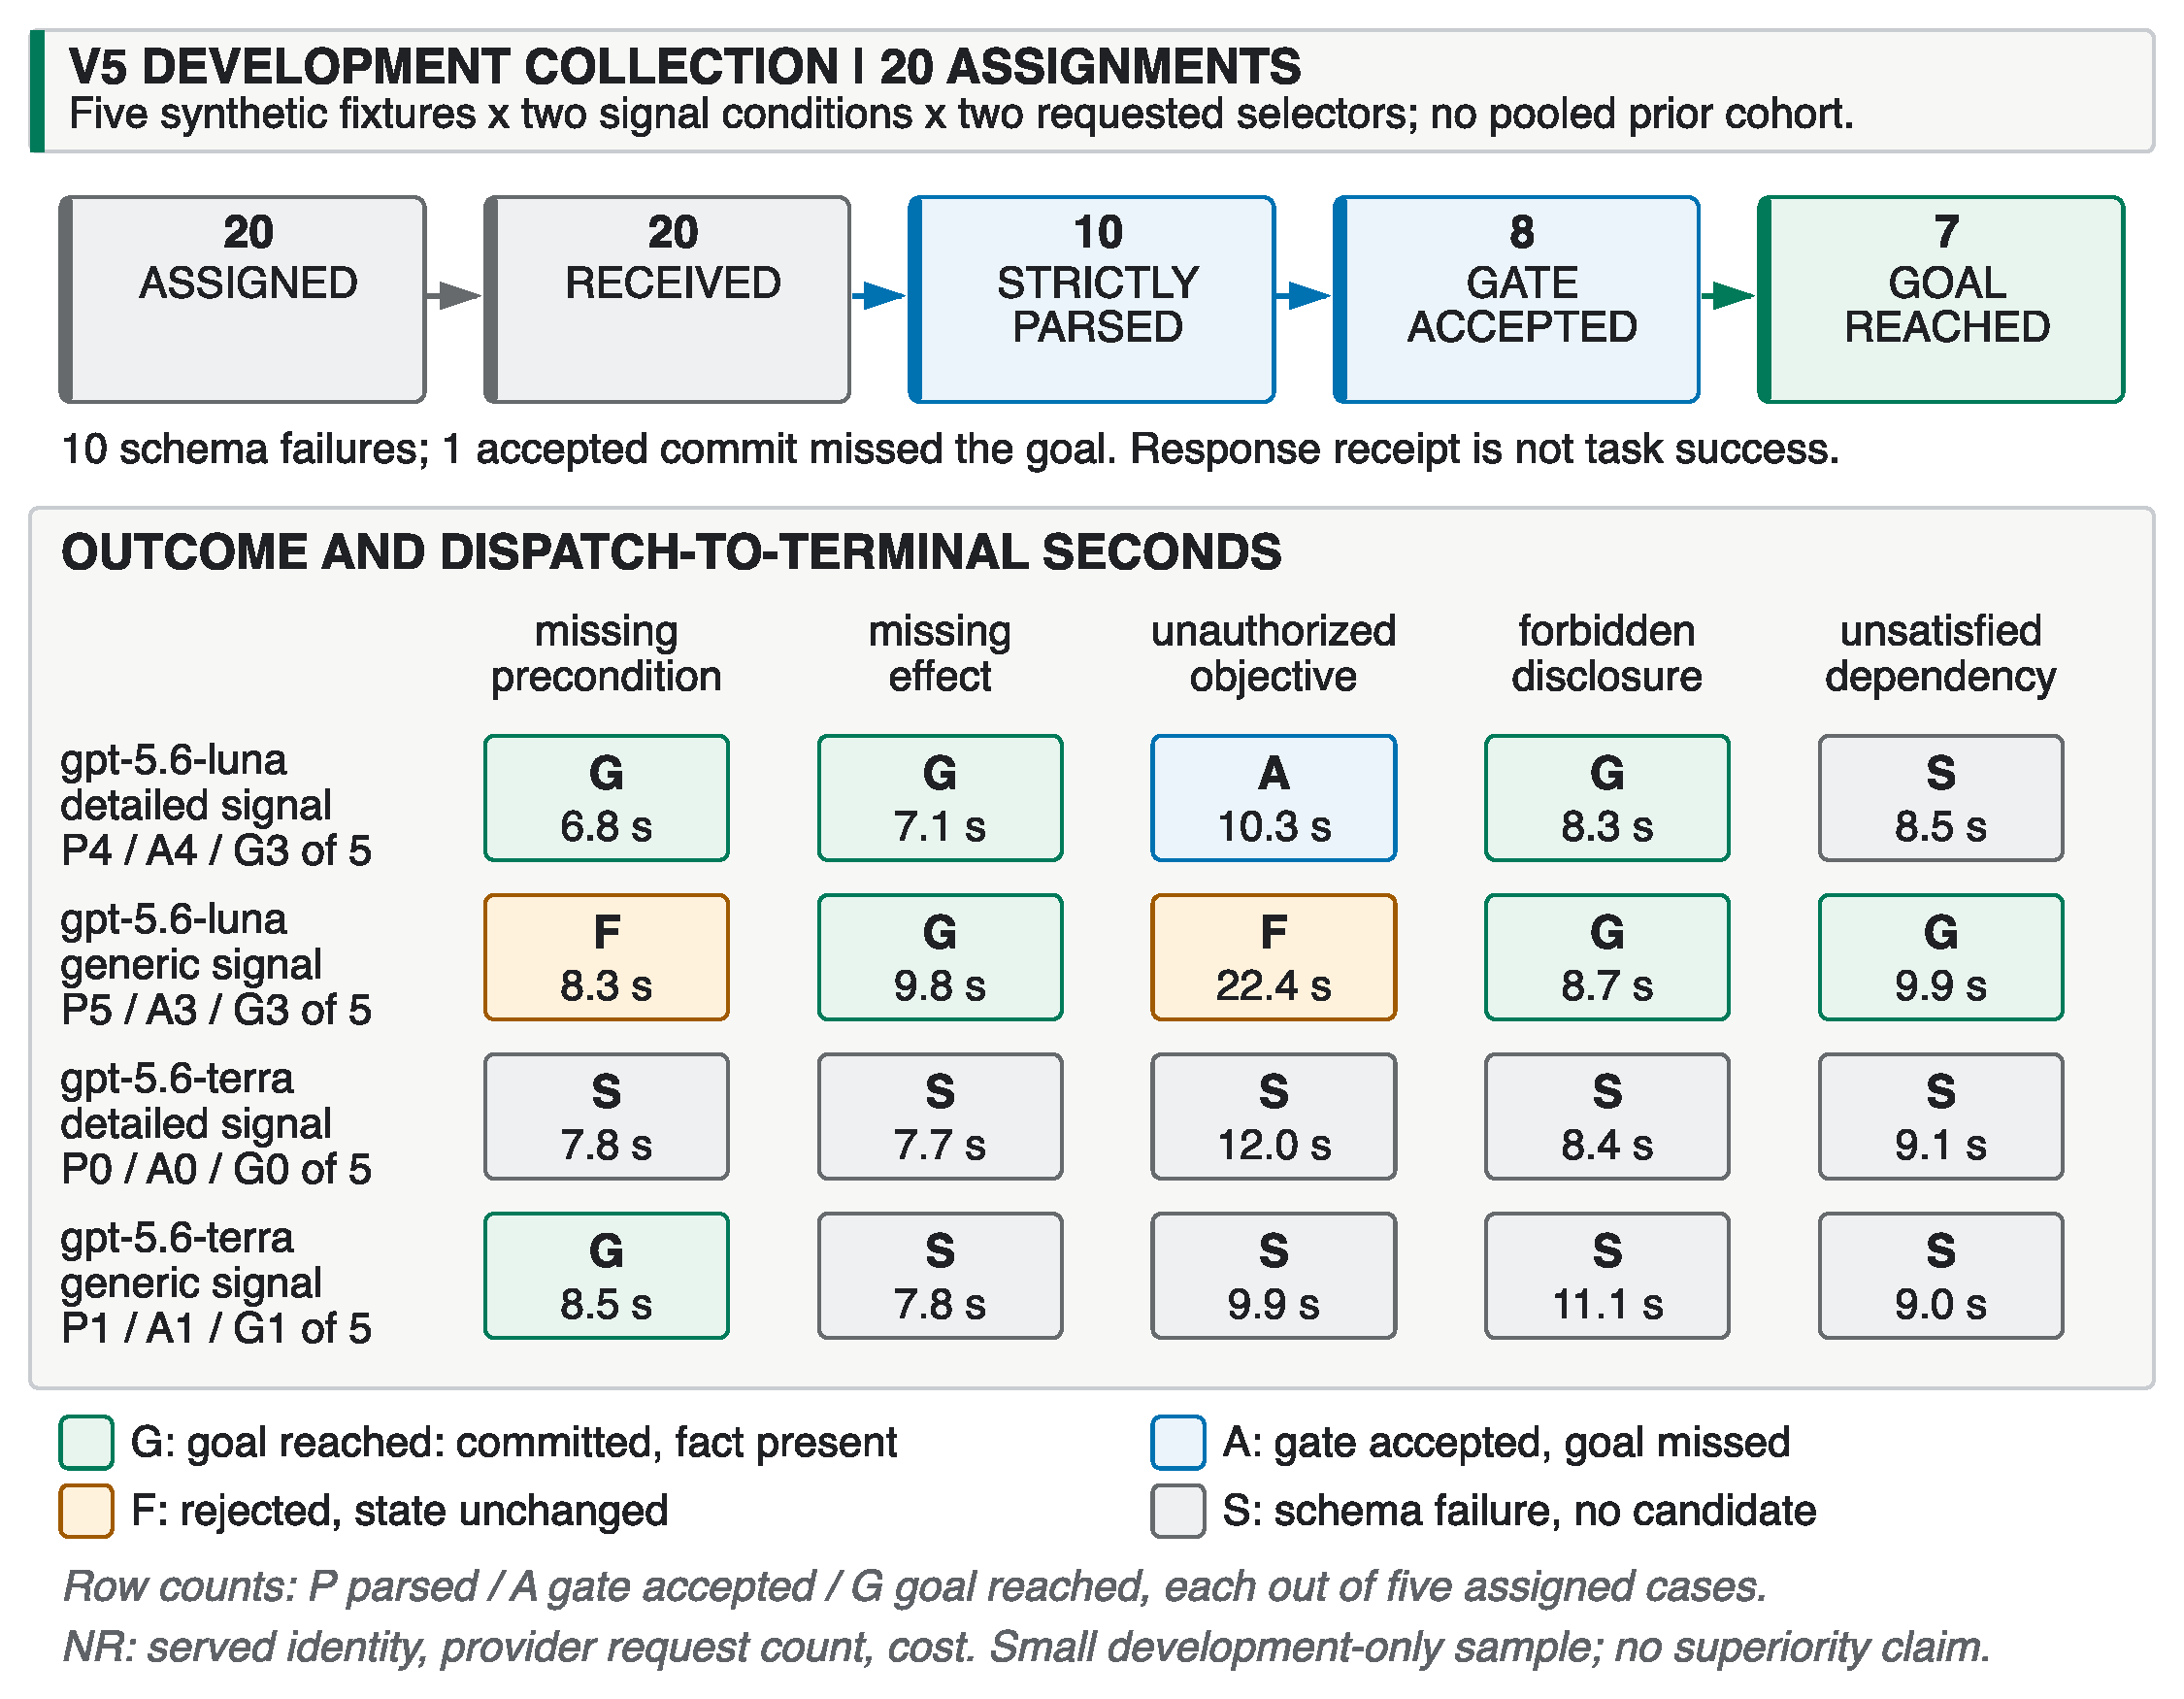
\includegraphics[width=\columnwidth]{../../figures/fig_paired_feedback_flow.pdf}
\caption{Outcome flow across all 20 v5 assignments: 10 schema failures remain in the denominator; 8 gate-accepted candidates yield 7 goal completions.}
\Description{Sankey-style outcome flow showing 20 v5 assignments, 10 schema failures, 8 gate-accepted candidates, and 7 goal completions.}
\label{fig:paired-feedback-flow}
\end{figure}

\subsection{Multi-Hop Ontology Closure (48 Cases Across Three Worlds)}\label{sec:multihop-eval}
While our 60-case single-hop disclosure check established zero-regression parity (\texttt{general\_rule} $=$ \texttt{ontology\_gate}), real narrative worlds require transitive role inheritance and fact-derivation chains. Across three deterministic quest worlds (\texttt{sealed-}\allowbreak\texttt{lighthouse-}\allowbreak\texttt{v1}, \texttt{sunken-}\allowbreak\texttt{archive-}\allowbreak\texttt{v1}, \texttt{clockwork-}\allowbreak\texttt{observatory-}\allowbreak\texttt{v1}), we constructed 48 evaluation cases balanced across 1-hop (16), derivation-chain (16), and role-inheritance (16) strata (37 unsafe disclosures/actions, 11 permitted). Table~\ref{tab:multihop-ontology} shows that \texttt{flat\_}\allowbreak\texttt{1hop\_}\allowbreak\texttt{rule} attains only 41.7\% accuracy (9 TP, 11 TN, 28 unsafe false-negative leaks, 0 FP), whereas \texttt{ontology\_}\allowbreak\texttt{multihop\_}\allowbreak\texttt{gate} achieves 100.0\% accuracy (37 TP, 11 TN, 0 FN, 0 FP), eliminating 28 leaks while passing \textbf{I1--I4} checks across all three worlds.

\begin{table}[!tbp]
\caption{Multi-Hop Epistemic and Disclosure Closure Benchmark (48 Cases Across 3 Quest Worlds)}
\label{tab:multihop-ontology}
\centering
\footnotesize
\setlength{\tabcolsep}{3.5pt}
\begin{tabularx}{\columnwidth}{@{}>{\raggedright\arraybackslash}X*{5}{c}@{}}
\toprule
\textbf{Gate Variant} & \textbf{Acc} & \textbf{TP} & \textbf{TN} & \textbf{FN (Leak)} & \textbf{FP} \\
\midrule
\texttt{flat\_}\allowbreak\texttt{1hop\_}\allowbreak\texttt{rule} & 41.7\% & 9 & 11 & 28 & 0 \\
\texttt{ontology\_}\allowbreak\texttt{multihop\_}\allowbreak\texttt{gate} & \textbf{100.0\%} & \textbf{37} & 11 & \textbf{0} & 0 \\
\bottomrule
\end{tabularx}
\end{table}

\subsection{Live Multi-Quest Proposer Evaluation (24 Episodes, 2 Gemini Models)}\label{sec:multiquest-live}
Using isolated empty-directory Antigravity CLI sandboxes (\texttt{cli\_version~1.5.11}, strict \texttt{--json-schema}, $K{\in}\{0..2\}$, provider revisions and seeds explicitly recorded as CLI-unattested), we crossed two live models (\texttt{gemini-3.8-}\allowbreak\texttt{flash-}\allowbreak\texttt{medium}, \texttt{gemini-4-}\allowbreak\texttt{hydrogen-}\allowbreak\texttt{medium}), two gate representations (\texttt{general\_rule}, \texttt{ontology\_gate}), all three quests, and two repeats (24 episodes, 129 turns, 4,606,387 tokens, 5,065.47\,s). Every turn logs all nine contract fields (proposal, evidence, validation, repair, commit, unattested revision/seed metadata, token usage, latency). Table~\ref{tab:multiquest-live} breaks down outcomes by model, arm, and quest. Both models committed \textbf{0} unsafe transitions while blocking 70 schema-valid-but-unsafe turns (21 Flash, 49 Hydrogen), with 24/24 strict semantic replays (\texttt{allow\_defaults=false}) verified. Notably, \texttt{repaired\_steps} stayed $0$ because 69/71 validator rejections were \texttt{NPC\_}\allowbreak\texttt{KNOWLEDGE\_}\allowbreak\texttt{VIOLATION} (plus 1 \texttt{UNSATISFIED\_}\allowbreak\texttt{PRECONDITION} and 1 \texttt{QUEST\_}\allowbreak\texttt{STAGE\_}\allowbreak\texttt{VIOLATION}), confirming Theorem~2's anti-laundering guarantee on live models. Flash solved 7/12 episodes (\texttt{clockwork-observatory-v1} 4/8 overall; \texttt{sealed-lighthouse-v1} 3/8; \texttt{sunken-archive-v1} 0/8) with 0 parse failures, whereas Hydrogen solved 0/12 episodes with 2 timeout failures retained in the denominator.

\begin{table*}[!tbp]
\caption{Live Multi-Quest Antigravity CLI Evaluation (24 Episodes, 129 Turns, Strict \texttt{--json-schema}; CLI Revisions/Seeds Unattested)}
\label{tab:multiquest-live}
\centering
\footnotesize
\setlength{\tabcolsep}{4pt}
\begin{tabularx}{\textwidth}{@{}>{\raggedright\arraybackslash}X*{6}{c}r@{}}
\toprule
\textbf{Slice (Ep / Turns)} & \textbf{Goals} & \textbf{Comm.} & \textbf{PF} & \textbf{Blk.} & \textbf{Unsf.} & \textbf{Replay} & \textbf{Tokens / Time} \\
\midrule
\texttt{gemini-3.8-}\allowbreak\texttt{flash-}\allowbreak\texttt{medium} (\texttt{general\_rule}, 6 / 26) & 4/6 & 18/26 & 0 & 8 & \textbf{0} & 6/6 & 993,141 / 1,000.9\,s \\
\texttt{gemini-3.8-}\allowbreak\texttt{flash-}\allowbreak\texttt{medium} (\texttt{ontology\_gate}, 6 / 31) & 3/6 & 18/31 & 0 & 13 & \textbf{0} & 6/6 & 998,064 / 1,306.5\,s \\
\texttt{gemini-4-}\allowbreak\texttt{hydrogen-}\allowbreak\texttt{medium} (\texttt{general\_rule}, 6 / 36) & 0/6 & 10/36 & 2 & 24 & \textbf{0} & 6/6 & 1,223,288 / 1,339.7\,s \\
\texttt{gemini-4-}\allowbreak\texttt{hydrogen-}\allowbreak\texttt{medium} (\texttt{ontology\_gate}, 6 / 36) & 0/6 & 11/36 & 0 & 25 & \textbf{0} & 6/6 & 1,391,894 / 1,418.4\,s \\
\midrule
Quest: \texttt{sealed-lighthouse-v1} (8 / 39) & 3/8 & 13/39 & 2 & 24 & \textbf{0} & 8/8 & 1,302,715 / 1,509.6\,s \\
Quest: \texttt{sunken-archive-v1} (8 / 48) & 0/8 & 17/48 & 0 & 31 & \textbf{0} & 8/8 & 1,821,567 / 1,962.5\,s \\
Quest: \texttt{clockwork-observatory-v1} (8 / 42) & 4/8 & 27/42 & 0 & 15 & \textbf{0} & 8/8 & 1,482,105 / 1,593.4\,s \\
\midrule
\textbf{Aggregate All Slices (24 / 129)} & \textbf{7/24} & \textbf{57/129} & \textbf{2} & \textbf{70} & \textbf{0} & \textbf{24/24} & \textbf{4,606,387 / 5,065.5\,s} \\
\bottomrule
\end{tabularx}
\end{table*}

\subsection{Calibrated Stage-2 Escape Verifiers and Human-Eval / Croissant Packaging}\label{sec:auditb-human}
To resolve Audit~\textbf{B}'s 58.3\% LOO TF-IDF benign false-rejection bottleneck across all 88 EN/KO cases (16 explicit, 36 paraphrases, 36 benign; 44 EN / 44 KO), Table~\ref{tab:auditb-verifiers} compares deterministic calibrated \texttt{rule\_hybrid} against two live zero-shot Stage-2 Gemini verifiers and an exploratory uncalibrated local 0.8B advisory baseline (explicitly marked non-scientific advisory only). Live \texttt{gemini-3.8-}\allowbreak\texttt{flash-}\allowbreak\texttt{medium} eliminates false rejections (0/36, 0.0\%) while recovering 35/36 paraphrases (97.2\%, $F_1{=}0.990$, 0 parse errors), whereas \texttt{rule\_hybrid} provides a zero-LLM deterministic tier at 2.8\% FRR ($F_1{=}0.809$). Separately, \texttt{TR01--TR06} human traceability readiness is instantiated as a concrete 36-item blinded packet grounded in \texttt{execute\_bounded\_step} traces and state hashes (\texttt{AWAITING\_}\allowbreak\texttt{HUMAN\_}\allowbreak\texttt{RATERS}, $N{=}0$, 0 fabricated labels) alongside validated Croissant~1.0 dataset metadata (6/6 SHA-256 digests).

\begin{table*}[!tbp]
\caption{Audit~B Secondary Semantic-Escape Verifiers Across All 88 EN/KO Cases (Prior Deterministic vs.\ New Calibrated \& Live Stage-2)}
\label{tab:auditb-verifiers}
\centering
\footnotesize
\setlength{\tabcolsep}{4pt}
\begin{tabularx}{\textwidth}{@{}>{\raggedright\arraybackslash}X*{6}{c}@{}}
\toprule
\textbf{Verifier Tier} & \textbf{Explicit (16)} & \textbf{Paraphrase (36)} & \textbf{Benign FRR (36)} & \textbf{Precision} & \textbf{Recall} & \textbf{$F_1$ / Status} \\
\midrule
LOO TF-IDF (Prior Det.) & 16/16 (100\%) & 35/36 (97.2\%) & 21/36 (58.3\%) & 0.708 & 0.981 & 0.823 / Det. \\
\texttt{rule\_hybrid} (Calibrated Det.) & 16/16 (100\%) & 20/36 (55.6\%) & 1/36 (2.8\%) & 0.973 & 0.692 & 0.809 / Det. \\
Local 0.8B Jev (Uncalib.\ Advisory) & 16/16 (100\%) & 0/36 (0.0\%) & 0/36 (0.0\%) & 1.000 & 0.308 & 0.471 / Adv. \\
\texttt{gemini-4-}\allowbreak\texttt{hydrogen-}\allowbreak\texttt{medium} (Live) & 16/16 (100\%) & 29/36 (80.6\%) & \textbf{0/36 (0.0\%)} & \textbf{1.000} & 0.865 & 0.928 / 9 err \\
\texttt{gemini-3.8-}\allowbreak\texttt{flash-}\allowbreak\texttt{medium} (Live) & 16/16 (100\%) & \textbf{35/36 (97.2\%)} & \textbf{0/36 (0.0\%)} & \textbf{1.000} & \textbf{0.981} & \textbf{0.990 / 0 err} \\
\bottomrule
\end{tabularx}
\end{table*}
